%% ============================================================================
%% IEEE conference paper (IEEEtran). Compile with pdfLaTeX (e.g. on Overleaf).
%% Figures live in ./figures/  (fig1..fig7 PNG). Fill TODO placeholders before
%% submission: co-author names/affiliations/ORCIDs and the repository URL.
%% Source of all numbers: data/artifacts/experiments/ + docs/dissertation/.
%% Note: 7 figures is a lot for a 6-page conference limit; trim if needed.
%% ============================================================================
\documentclass[conference]{IEEEtran}
\IEEEoverridecommandlockouts
\usepackage{cite}
\usepackage{amsmath,amssymb,amsfonts}
\usepackage{graphicx}
\usepackage{booktabs}
\usepackage{array}
\usepackage{textcomp}
\usepackage{xcolor}
\usepackage[hidelinks]{hyperref}

\begin{document}

\title{Does Feature Richness Help? A Reproducible, Honest Evaluation of a
Student Digital Twin and Its Explanation Stability Across Two Institutions}

\author{
\IEEEauthorblockN{Aibyn Talgat}
\IEEEauthorblockA{\textit{School of Software Engineering} \\
\textit{Astana IT University}\\
Astana, Kazakhstan \\
a1byn.talgat05@gmail.com \\
ORCID: 0000-0000-0000-0000}
\and
\IEEEauthorblockN{Co-author 2 \textit{(TODO)}}
\IEEEauthorblockA{\textit{Affiliation} \\
City, Country \\
email \\
ORCID: 0000-0000-0000-0000}
\and
\IEEEauthorblockN{Co-author 3 \textit{(TODO)}}
\IEEEauthorblockA{\textit{Affiliation} \\
City, Country \\
email \\
ORCID: 0000-0000-0000-0000}
}

\maketitle

\begin{abstract}
Learning management systems (LMS) record large volumes of educational activity,
but their built-in analytics are mostly descriptive rather than predictive or
explanatory. This paper presents a teacher-facing \textbf{Student Digital Twin}
--- a lean, time-aware weekly student-state representation --- coupled with an
\textbf{Explainable AI (XAI)} layer and an end-to-end interface that turns raw
public learning-analytics data into per-student grade predictions, pass-risk
flags, and model-behaviour explanations. Rather than reporting a single best
configuration, we run a dependency-driven sequence of frozen experiments and ask
a falsifiable question: \emph{do engineered Digital-Twin features improve
prediction over a competent LMS baseline, and are the explanations stable?} On
the Open University Learning Analytics Dataset (OULAD) module DDD~2013J
(1{,}938 students, 67{,}830 weekly snapshots) the full Twin ablation is
\textbf{mixed-to-null} --- no Twin block beats the LMS baseline by more than
$1.0$ RMSE --- while on a second cohort (BBB~2013J) a mastery block improves the
temporal-forward split by $-1.026$~RMSE but nothing else. A second institution
(KU~Leuven, 1{,}495 students) cannot even support the mastery ablation. Across
three real cohorts and two institutions, \textbf{adding feature richness does not
robustly help}, and the XAI importance rankings are regime-sensitive (Kendall
$\tau$ 0.55--0.79 within a course, 0.32--0.61 across courses). The contribution
is a reproducible, leakage-aware prototype with a teacher UI and an honest,
multi-cohort evaluation --- including a documented synthetic-target circularity
failure mode --- rather than an accuracy record.
\end{abstract}

\begin{IEEEkeywords}
learning analytics, explainable AI, explanation stability, student performance
prediction, OULAD, digital twin, gradient boosting, permutation importance,
teacher-facing dashboards, reproducibility, honest negative result
\end{IEEEkeywords}

\section{Introduction}
Learning management systems capture attendance, submissions, marks, and
clickstream activity, yet teachers still lack an integrated, forward-looking
view of a student's evolving academic state, the likely end-of-course outcome,
and the factors behind that estimate. Most published learning-analytics work
optimises a classifier for accuracy on a held-out split and appends post-hoc
explanations, reporting only the best configuration on a single cohort. This
leaves three practical questions unanswered: whether a \emph{Digital-Twin}
representation of student state adds defensible value over a plain LMS feature
set, whether the resulting explanations are stable enough to show a teacher, and
whether the whole cycle can be implemented and reproduced on real public data.

This paper addresses those questions with a working prototype and an explicitly
honest evaluation. The central object is the student modelled as a
\textbf{dynamic digital twin}: weekly state snapshots at the grain
\emph{1 row = 1 student $\times$ 1 week}. The term ``Digital Twin'' here denotes
a lean, time-aware state representation, not a counterfactual or simulation
engine. We retain the term deliberately but scope it narrowly to a
\emph{descriptive} state twin, and treat the absence of a
simulation/counterfactual layer as an explicit design boundary
(Section~\ref{sec:limitations}) rather than an implicit promise. Around this
representation we build a gradient-boosting predictor, a perturbation-based XAI
layer, and a Next.js teacher interface that reads frozen prediction artifacts.

The novelty is not a new algorithm or a higher accuracy number. It is the
combination of (1)~an end-to-end, open, leakage-aware pipeline from raw OULAD
data to teacher-facing weekly explanations; (2)~a dependency-driven ablation that
tests the Twin representation instead of assuming it; (3)~an explanation-stability
analysis across splits, courses, and institutions; and (4)~an \textbf{honest
multi-cohort finding} --- including a documented synthetic-data circularity
failure mode --- of a kind systematically underrepresented in the literature.

\section{Related Work}
\textbf{SHAP + gradient boosting on OULAD.} Training gradient boosting or random
forests on OULAD and adding SHAP explanations post-hoc is now standard practice
\cite{lopez2025,review2026,xai2025,frontiers2025}. Published benchmarks reach
ROC-AUC 0.993 and F1 0.911 on dropout prediction \cite{lopez2025}. Adding
explainability is therefore no longer a contribution by itself, and
continuous-grade regression --- used here alongside classification --- is
comparatively less common but not sufficient on its own.

\textbf{Explanation stability.} Tiukhova et al.\ \cite{tiukhova2024} showed that
XAI-derived feature importance for student-success models can be unstable across
configurations. We extend this stability lens from the single-model setting to a
\emph{transfer} setting, measuring rank agreement across evaluation splits,
across two OULAD courses, and across institutions.

\textbf{Digital Twin in education.} Digital twins in education appear mostly as
conceptual or review work \cite{dt2022}; working implementations of a student
digital twin on real data are essentially absent. Teacher-facing interfaces in
peer-reviewed work publish model metrics, not systems; commercial platforms (EAB
Navigate, Civitas Learning, Brightspace Insights) have dashboards but are closed
and undocumented. Papers that add SHAP rarely address how teachers may
\emph{misinterpret} explanations or the difference between model-behaviour
description and causal claim.

\textbf{Research gap.} No published work implements and honestly evaluates a
full-cycle prototype --- raw data $\rightarrow$ weekly twin snapshots
$\rightarrow$ predictions $\rightarrow$ per-student explanations $\rightarrow$
teacher UI --- on real public data, with explicit documentation of where the
added components fail to beat a simpler baseline. This paper targets that gap.

\section{System Architecture}
The prototype is a monorepo with two independently runnable services and a strict
read-only boundary between computation and presentation.

\textbf{ML service (\texttt{services/ml}, Python).} Contains the OULAD data
adapter, the weekly snapshot builder, the feature-engineering pipeline, the
experiment runner, the model-training code, and the perturbation-based XAI
module. All experiment outputs are versioned JSON/CSV artifacts under
\texttt{data/artifacts/experiments/}.

\textbf{Web service (\texttt{apps/web}, Next.js).} A server-side-rendered
frontend that reads the frozen artifacts at request time and serves
teacher-facing views. It performs no ML computation, so results are reproducible
independently of the UI and the UI is testable without retraining.

\textbf{Data flow.} Raw OULAD CSV $\rightarrow$ OULAD adapter $\rightarrow$ weekly
snapshot table (one row per student per week) $\rightarrow$ feature engineering
$\rightarrow$ trained Gradient Boosting model $\rightarrow$ prediction +
perturbation-based explanation artifacts $\rightarrow$ JSON consumed by the web
app (Fig.~\ref{fig:arch}).

\begin{figure*}[!t]
\centering
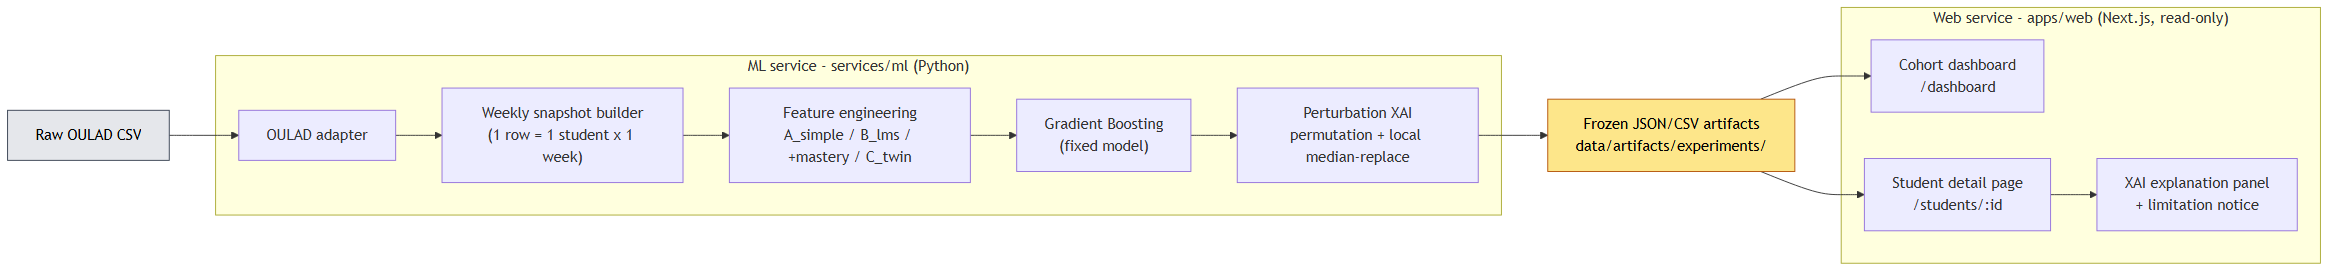
\includegraphics[width=\textwidth]{figures/fig1_architecture.png}
\caption{End-to-end architecture: raw OULAD CSV $\rightarrow$ ML service (adapter
$\rightarrow$ weekly snapshots $\rightarrow$ feature engineering $\rightarrow$
Gradient Boosting $\rightarrow$ XAI) $\rightarrow$ frozen JSON artifacts
$\rightarrow$ read-only Next.js teacher interface.}
\label{fig:arch}
\end{figure*}

\textbf{Teacher interface.} A \emph{cohort dashboard} (Fig.~\ref{fig:dash})
presents a sortable, filterable table of all students with predicted grade,
pass-risk badge, current week, and key LMS signals. A \emph{student detail page}
(Fig.~\ref{fig:detail}) shows summary cards (predicted vs.\ actual grade, risk,
mastery, activity, attendance, assignment/quiz averages, 3-week trend), a weekly
trajectory chart, a raw weekly-snapshot table, and an explanation panel listing
which signals raise or lower the current-week prediction. The panel carries an
explicit XAI limitation notice: the factors describe \emph{model behaviour, not
causes}; the score is not a sole basis for intervention; and rankings can shift
across time periods and cohorts. This framing directly operationalises the
research gap of Section~II. We present the interface as a \emph{design
demonstrator} whose presentation of XAI output is derived from the
explanation-stability result (Section~\ref{sec:xai}), not as an evaluated
intervention; no user study is claimed here.

\begin{figure*}[!t]
\centering
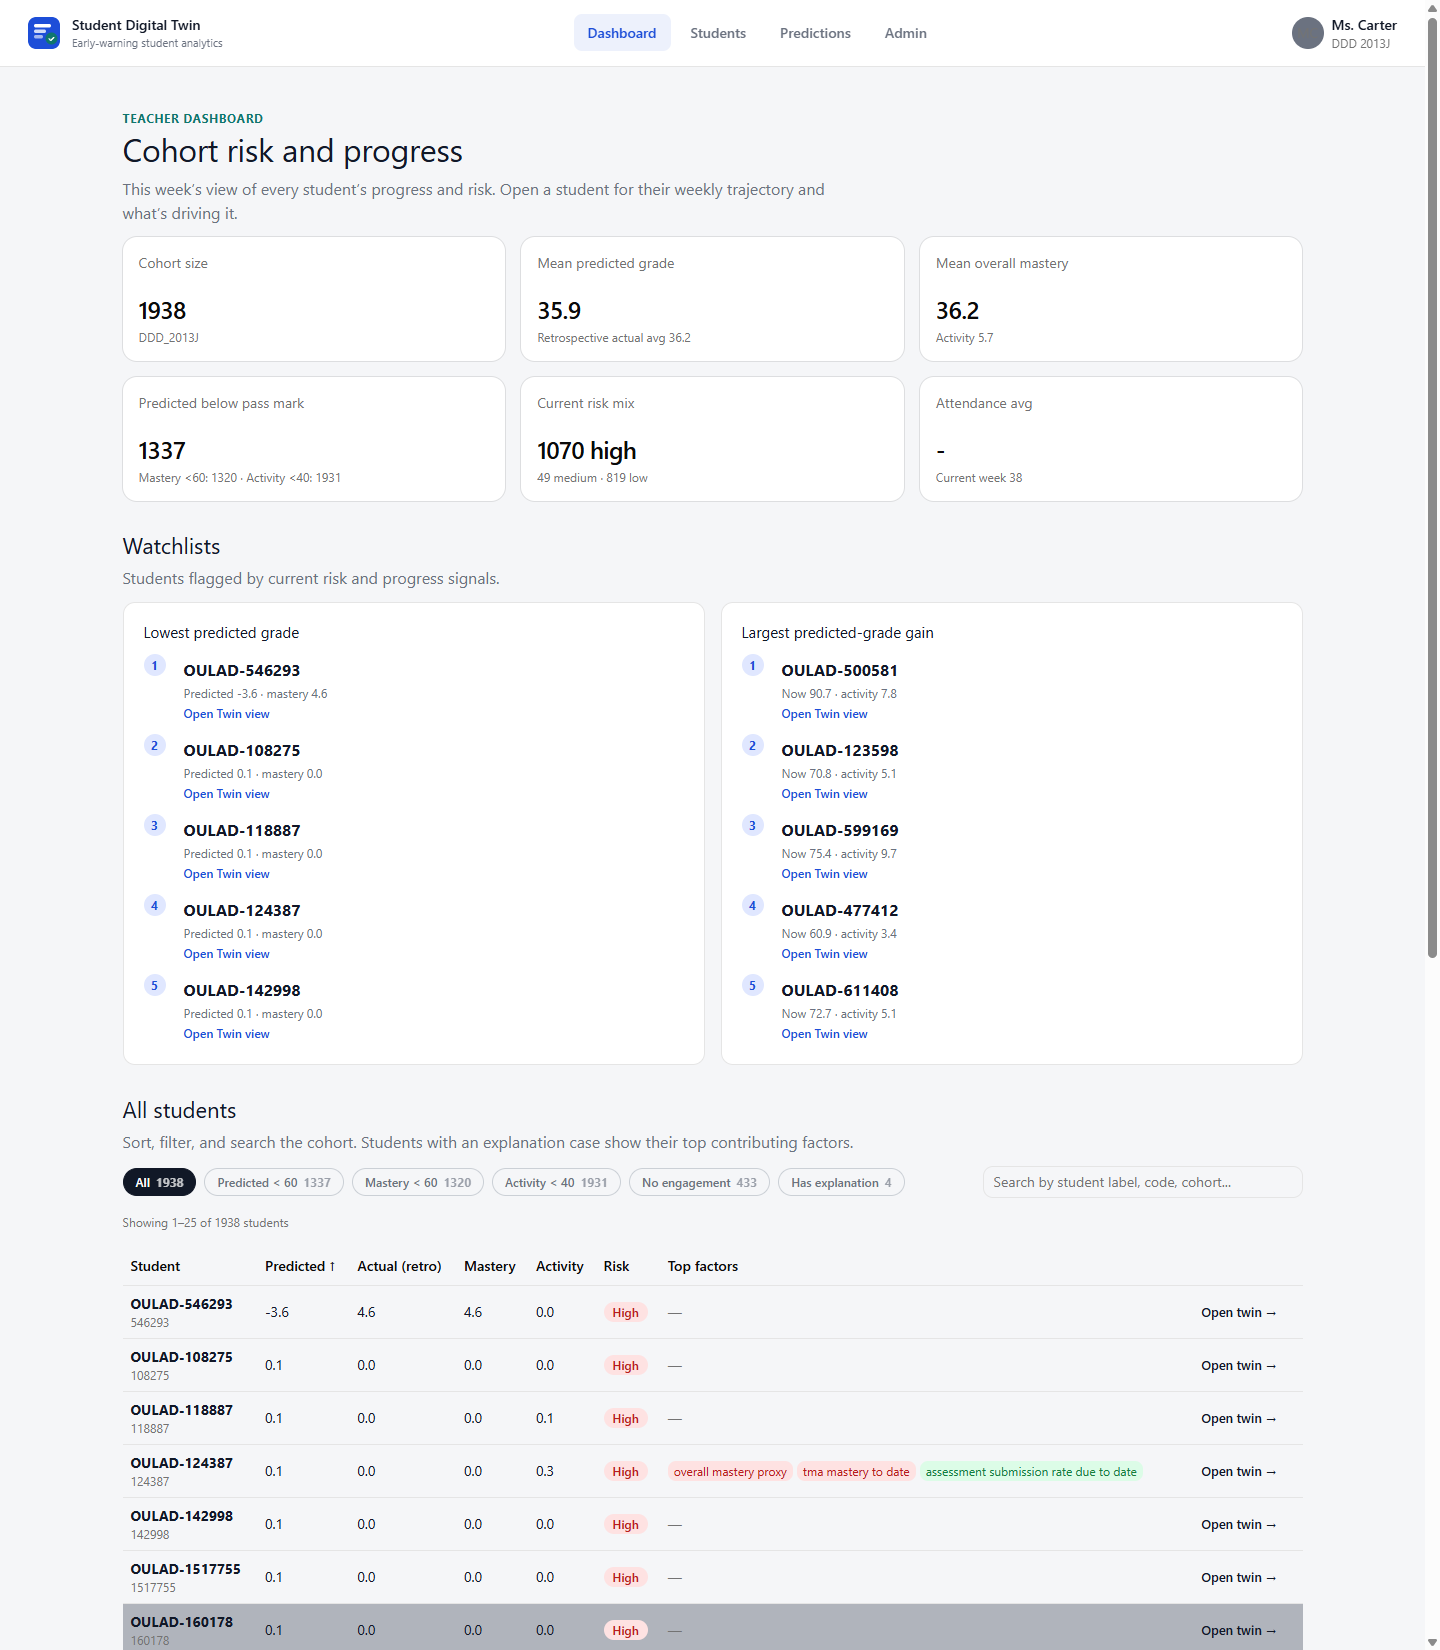
\includegraphics[width=0.92\textwidth]{figures/fig2_dashboard.png}
\caption{Teacher cohort dashboard: a sortable, filterable table of all students
with predicted final grade, pass-risk badge (high / medium / low), current week,
and key LMS signals, supporting one-click filtering to the high-risk group.}
\label{fig:dash}
\end{figure*}

\begin{figure*}[!t]
\centering
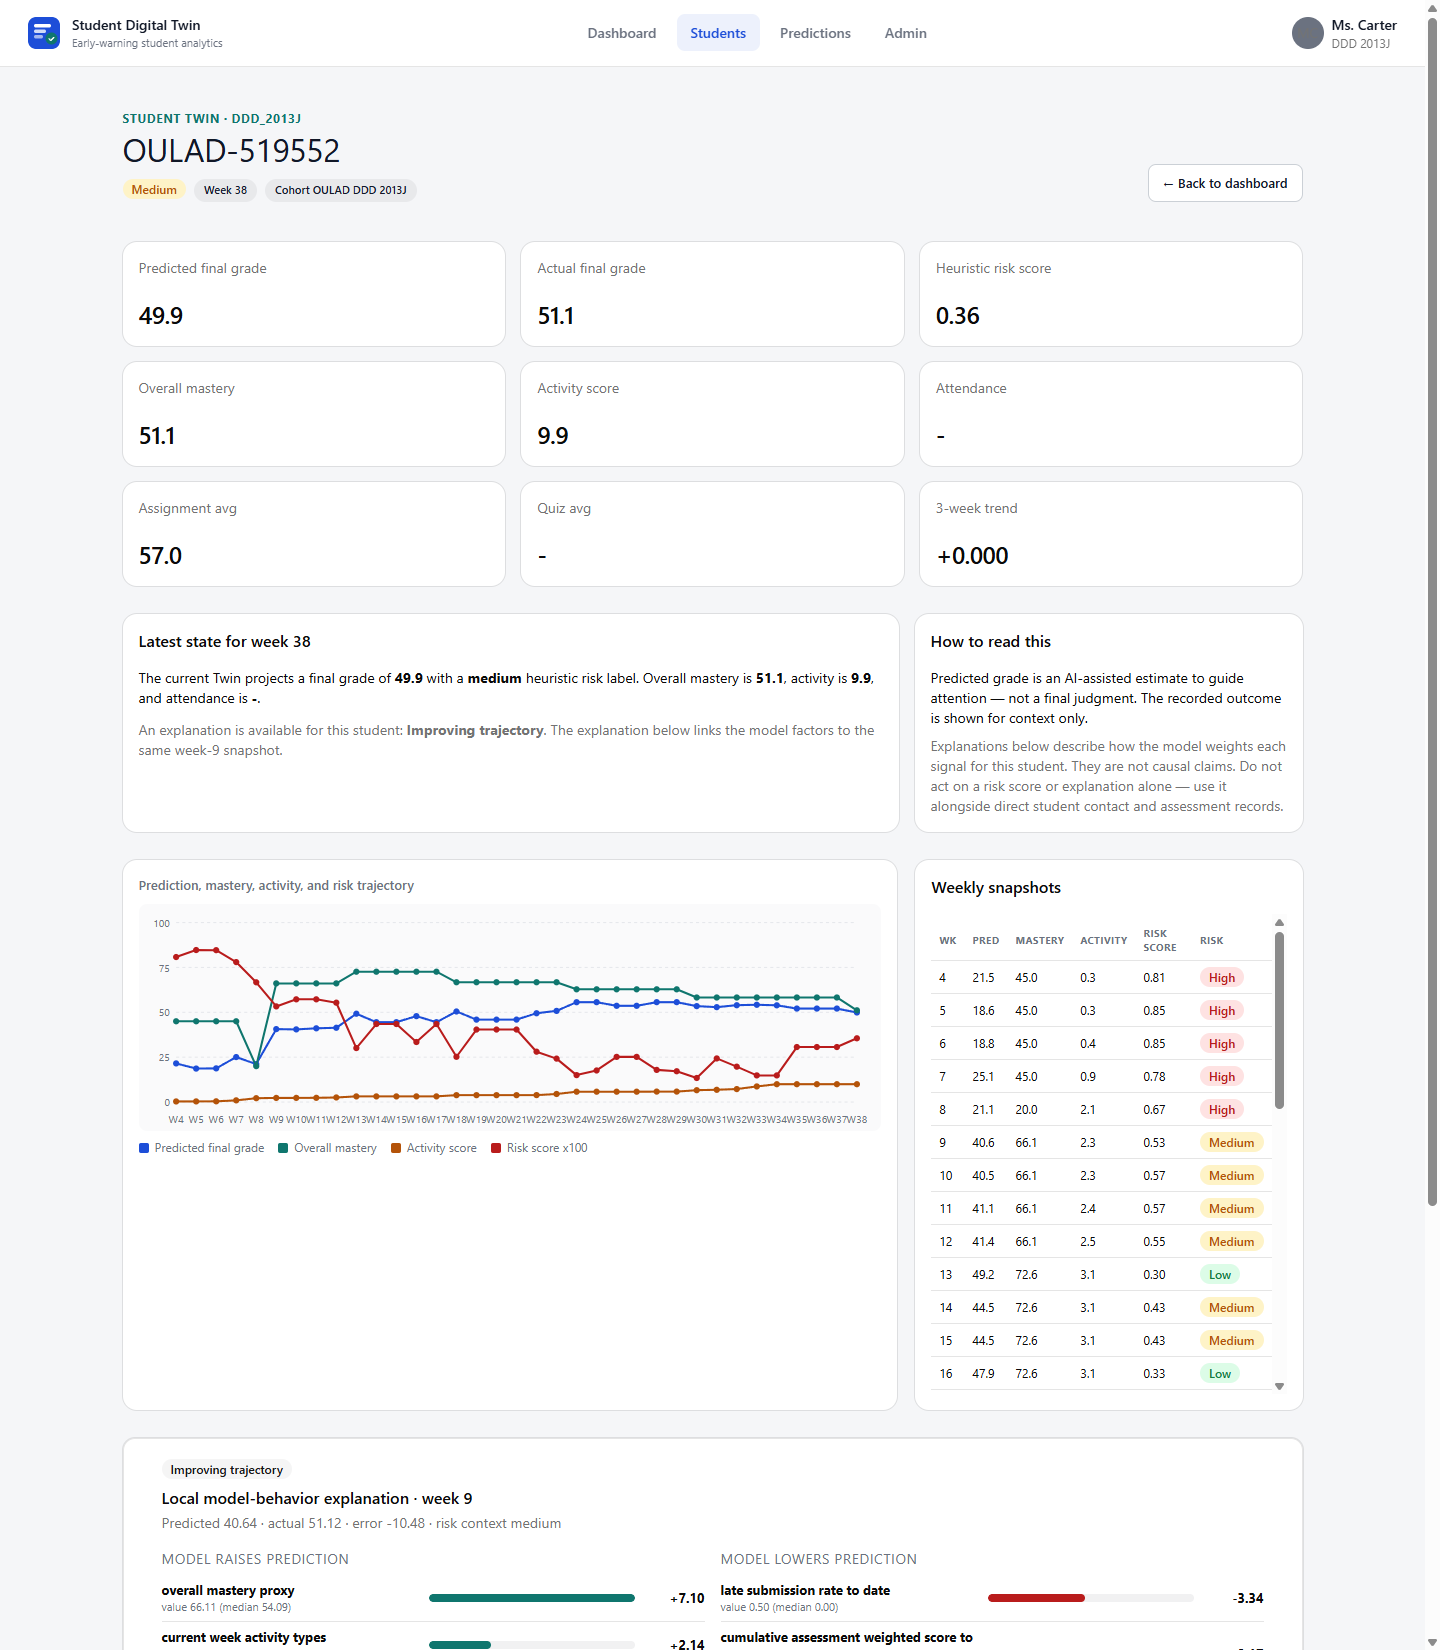
\includegraphics[width=0.92\textwidth]{figures/fig3_student_detail.png}
\caption{Per-student view: summary cards (predicted vs.\ actual grade, risk,
mastery, activity, attendance, assignment/quiz averages, 3-week trend), the
weekly trajectory chart, and the raw weekly-snapshot table.}
\label{fig:detail}
\end{figure*}

\section{Data and Experimental Design}
\subsection{Datasets}
We evaluate on real, public, non-circular data from two institutions.
\begin{itemize}
\item \textbf{OULAD DDD 2013J} \cite{kuzilek2017}: 1{,}938 students, 67{,}830
weekly snapshots, weeks 4--38.
\item \textbf{OULAD BBB 2013J} \cite{kuzilek2017}: 2{,}237 students, 80{,}532
weekly snapshots; richer dated assessment structure than DDD.
\item \textbf{KU Leuven 1819} \cite{tiukhova2026}: 1{,}495 students, two courses
pooled, weeks 2--15.
\end{itemize}
A separate \textbf{synthetic} dataset is used only for controlled methodological
checks; its limitations are stated in Section~\ref{sec:limitations}.

\subsection{Feature sets (nested ablation)}
The Digital-Twin representation is tested by decomposition, not assumed
(Fig.~\ref{fig:ablation}):
\begin{itemize}
\item \texttt{A\_simple} --- minimal baseline.
\item \texttt{B\_lms} --- LMS behavioural features (the proxy for ``what the
literature uses'').
\item \texttt{B\_lms + mastery} --- LMS plus a lean mastery-proxy block derived
from the dated assessment structure.
\item \texttt{C\_twin} --- full engineered Twin representation (trends, mastery,
indices, temporal context).
\end{itemize}

\begin{figure}[!t]
\centering
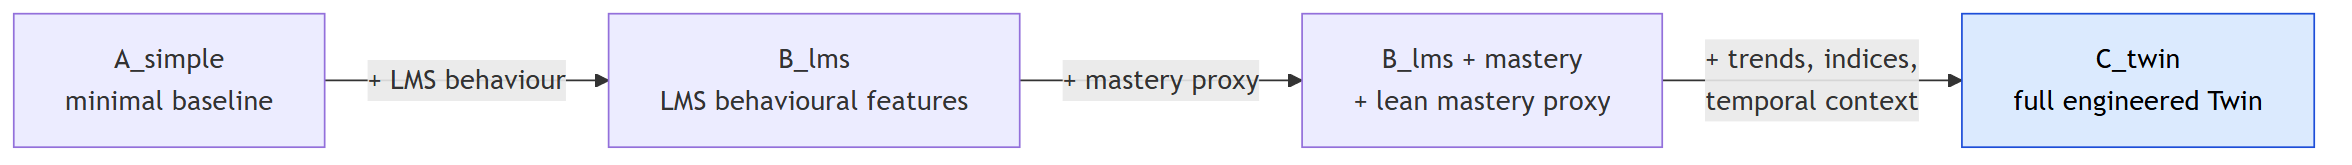
\includegraphics[width=\columnwidth]{figures/fig4_ablation.png}
\caption{Nested feature-set ablation. Each set is a strict superset of the
previous one (\texttt{A\_simple} $\subset$ \texttt{B\_lms} $\subset$
\texttt{B\_lms+mastery} $\subset$ \texttt{C\_twin}), so the Digital-Twin
representation is tested by decomposition rather than assumed.}
\label{fig:ablation}
\end{figure}

\subsection{Models and protocol}
Model families are deliberately simple and defensible: Ridge regression, Logistic
Regression, Random Forest, and Gradient Boosting. Two splits are used: a
\textbf{student-grouped} split (primary; \texttt{test\_size}~$=0.25$,
\texttt{seed}~$=42$; for DDD: 1{,}454 train vs.\ 484 test students) and a
\textbf{temporal-forward} split (train on early weeks, predict later weeks). The
pipeline is leakage-aware: train-only preprocessing, explicit forbidden-column
enforcement, and \textbf{fixed-model} reporting (Gradient Boosting held fixed
across splits) to neutralise best-model-per-cell selection artifacts. Targets:
\texttt{final\_weighted\_score} (regression, 0--100) and
\texttt{passed\_observed} (binary classification).

\section{Results}
\subsection{This work vs.\ standard baselines}
All rows in Table~\ref{tab:compare} use OULAD DDD 2013J, the \texttt{B\_lms}
feature set, and the student-grouped split, except the last ``ours'' row which
adds the mastery block. RMSE is on the 0--100 score scale; F1/ROC-AUC are for
\texttt{passed\_observed}.

\begin{table*}[!t]
\caption{This work vs.\ standard baselines and published references on OULAD DDD
2013J (student-grouped split).}
\label{tab:compare}
\centering
\footnotesize
\begin{tabular}{lcccccc}
\toprule
Approach & RMSE & F1 & ROC-AUC & Per-student XAI & Teacher UI & Open \\
\midrule
Logistic Regression (ours) & --- & 0.854 & 0.951 & No & No & Yes \\
Random Forest (ours) & 13.633 & 0.861 & 0.947 & No & No & Yes \\
GB LMS-only (ours) & 12.658 & 0.863 & 0.953 & No & No & Yes \\
\textbf{GB + Twin + XAI (this work)} & \textbf{12.724} & \textbf{0.861} & \textbf{0.953} & \textbf{Yes (perturbation)} & \textbf{Yes} & \textbf{Yes} \\
GB + SHAP (literature) \cite{lopez2025} & --- & 0.911 & 0.993 & Yes (SHAP) & No & Partial \\
Commercial (EAB Navigate) & unknown & unknown & unknown & Partial & Yes & No \\
\bottomrule
\end{tabular}
\end{table*}

Gradient Boosting on \texttt{B\_lms} is the strongest baseline (RMSE 12.658,
F1 0.863, ROC-AUC 0.953); Ridge regression is the weakest (RMSE 14.318). Logistic
Regression is already competitive (F1 0.854, ROC-AUC 0.951), reflecting that the
dominant predictor --- assessment submission rate --- is approximately linear in
the log-odds of passing. Adding the mastery (Twin) block changes RMSE by
$+0.066$ (worse) and F1 by $-0.002$: no improvement on this cohort and split.
This is the honest negative result, stated rather than hidden.

\subsection{When does the Twin help, and when not?}
The full nested ablation under fixed-model reporting gives a course- and
split-dependent answer (Table~\ref{tab:twinhelp}).

\begin{table}[!t]
\caption{Mastery block vs.\ \texttt{B\_lms} (RMSE delta; lower is better).}
\label{tab:twinhelp}
\centering
\footnotesize
\begin{tabular}{lll}
\toprule
Cohort & Student-grouped & Temporal-forward \\
\midrule
DDD 2013J & null (mastery $+0.061$) & weak: mastery $-0.381$ \\
BBB 2013J & null (all within 0.087) & \textbf{largest gain: mastery $-1.026$} \\
\bottomrule
\end{tabular}
\end{table}

On DDD, no Twin block beats \texttt{B\_lms} by more than $1.0$ RMSE on either
split, the full \texttt{C\_twin} stays within $\pm0.025$ RMSE (non-inferior, not
better), and the minimal \texttt{A\_simple} is clearly worse ($+1.207$ grouped,
$+4.105$ temporal-forward) --- confirming the LMS layer already carries the
signal. On BBB, which has a richer assessment structure, the mastery block
improves the temporal-forward split by $-1.026$ RMSE ($6.311 \rightarrow 5.284$)
and the full \texttt{C\_twin} by $-0.765$, but the student-grouped split stays
null and the trend/index blocks are null on both courses.

\textbf{Reading.} Engineered Twin value is \emph{heterogeneous}: it appears only
under forward-time prediction on a course with rich assessment structure, and
disappears under the student-grouped regime. It is not a robust improvement. We
verified that the single positive cell is not noise: a student-clustered
bootstrap (5{,}000 resamples of the held-out test students) places the 95\%
confidence interval of the mastery RMSE reduction entirely below zero. The
magnitude is nonetheless sensitive to the out-of-time extrapolation regime, so we
treat this as the one cell where Twin features clearly help, not as a stable
effect size. Crucially, the OULAD classification target is genuinely predictive
throughout (best-model F1 0.83--0.93, never 1.000), which is what makes this
negative finding trustworthy. Fig.~\ref{fig:evalarc} summarises the arc.

\begin{figure*}[!t]
\centering
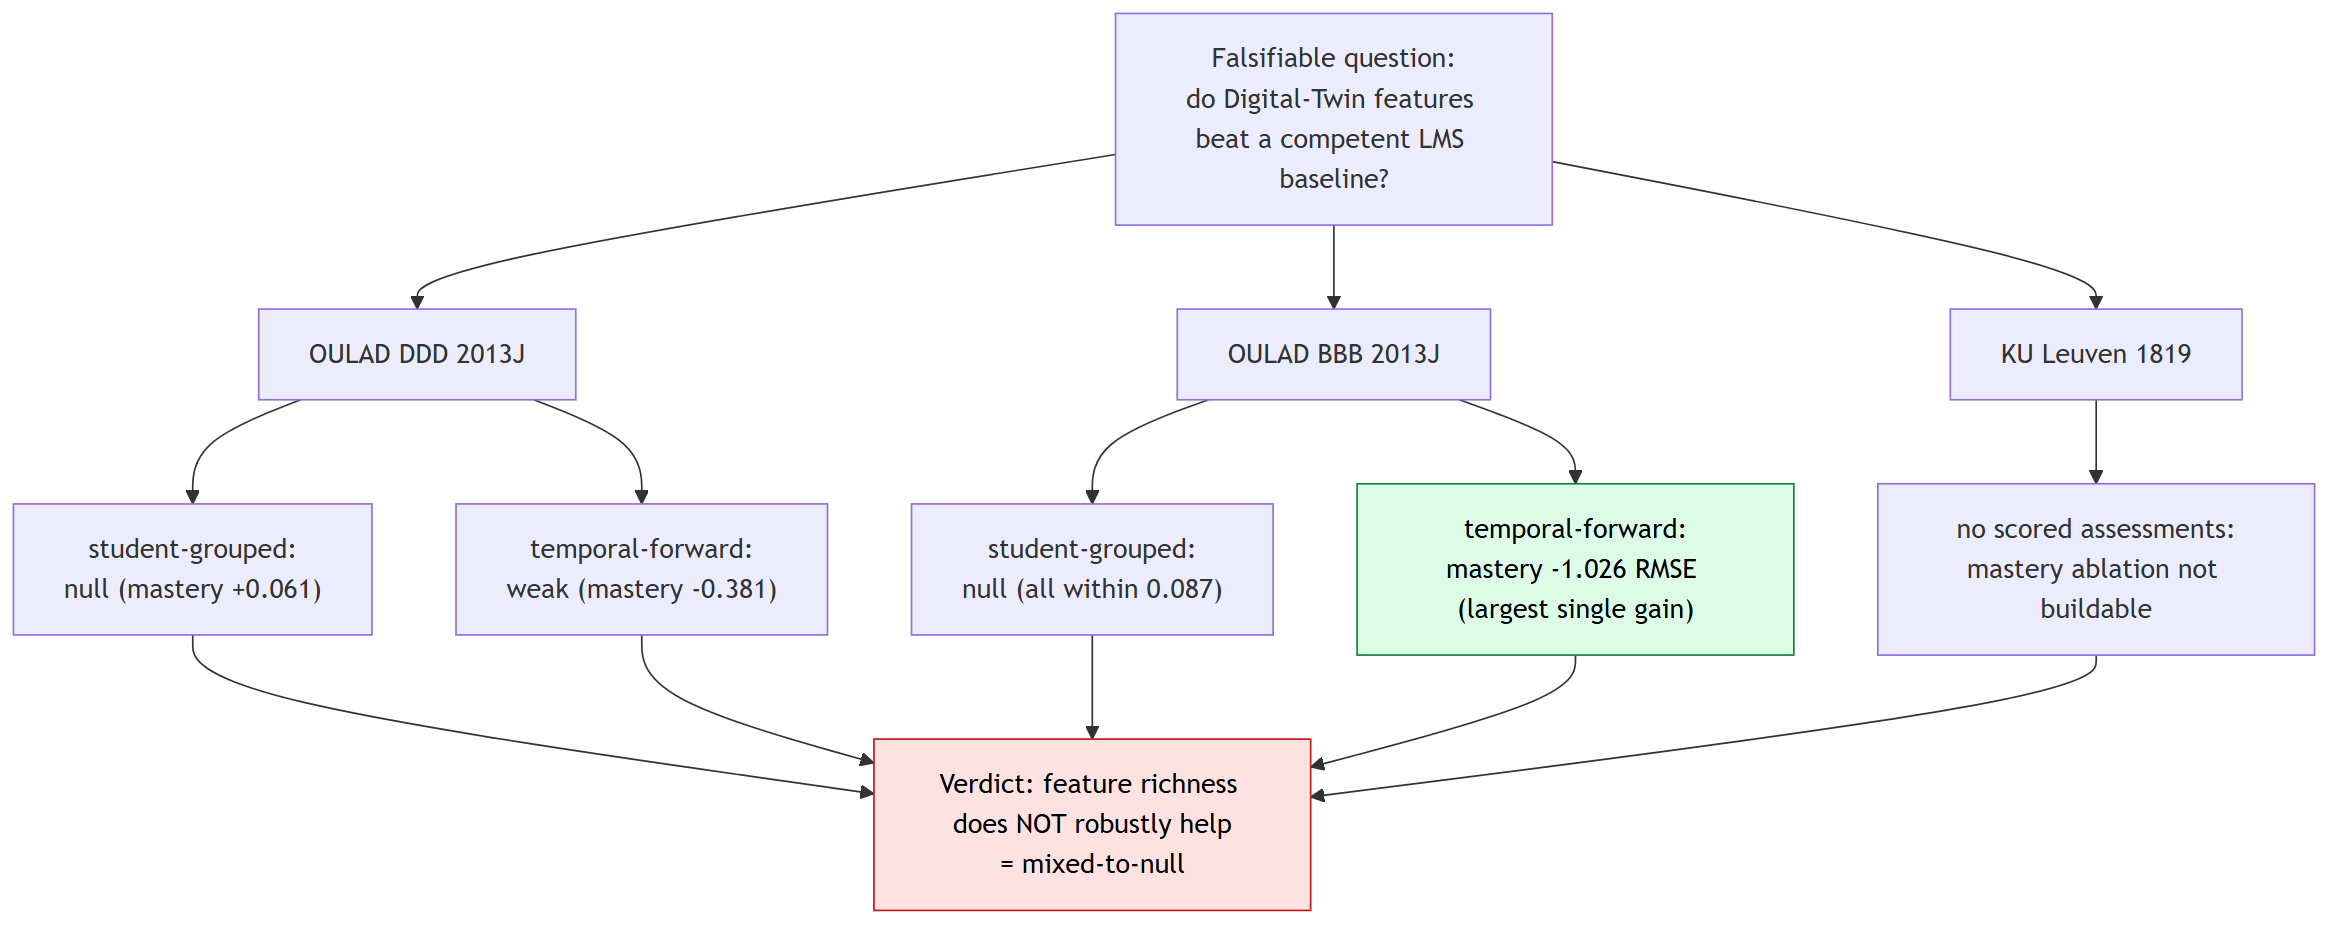
\includegraphics[width=\textwidth]{figures/fig5_evalarc.png}
\caption{Dependency-driven evaluation arc and its honest verdict: the falsifiable
question is tested across three real cohorts and two splits. Only the BBB
temporal-forward cell shows a real mastery gain ($-1.026$ RMSE); everything else
is null or weak, so the overall finding is mixed-to-null --- feature richness
does not robustly help.}
\label{fig:evalarc}
\end{figure*}

\subsection{XAI and explanation stability}
\label{sec:xai}
Explanations use held-out \textbf{permutation importance}, model-native
importance, and one-feature \textbf{local median-replacement} perturbation. We
deliberately avoid SHAP: Shapley-value attributions rest on a background /
conditional-expectation estimate that is fragile on the small per-student samples
surfaced in the teacher UI, and have documented conceptual and robustness
problems as feature-importance measures \cite{kumar2020,slack2020}; the
perturbation method instead operates directly on the single prediction row shown
to the teacher, with no background-set assumption. On DDD, the dominant factor is
\texttt{assessment\_submission\_rate\_due\_to\_date} (importance share 0.28--0.38;
0.381 in the headline model) and, once mastery is included, the co-circular
\texttt{overall\_mastery\_proxy} (0.23--0.43). The genuinely exogenous signals
--- \texttt{is\_unregistered\_by\_week} (0.13--0.20) and VLE clickstream
(0.02--0.06) --- are interpretable but carry modest weight (Fig.~\ref{fig:xai}).

\begin{figure}[!t]
\centering
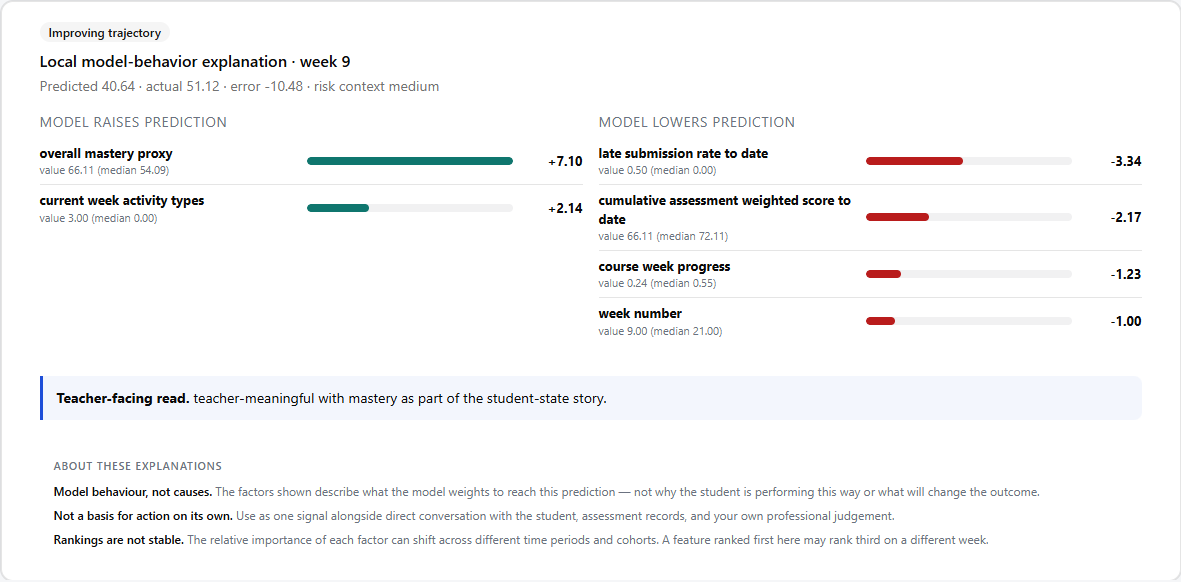
\includegraphics[width=\columnwidth]{figures/fig6_xai_panel.png}
\caption{Per-student model-behaviour explanation: signals that raise vs.\ lower
the current-week prediction, a teacher-readable summary sentence, and the
explicit XAI limitation notice (model behaviour, not causes; not a sole basis for
intervention; rankings shift across regimes).}
\label{fig:xai}
\end{figure}

The rankings are \textbf{not invariant}:
\begin{itemize}
\item \emph{Within a course, across splits:} Kendall $\tau = 0.79 / 0.68 / 0.55$
for \texttt{B\_lms} / \texttt{+mastery} / \texttt{C\_twin} (mean 0.67); none
reach 0.90.
\item \emph{Across courses (DDD vs.\ BBB):} $\tau = 0.32$--$0.61$ (mean 0.52) ---
even less stable.
\item \emph{Across three institutions (engagement-only):} mean $\tau \approx
0.56$; clicks and active-days recur as top drivers, but the mid/lower ordering is
institution-specific.
\end{itemize}

\begin{figure}[!t]
\centering
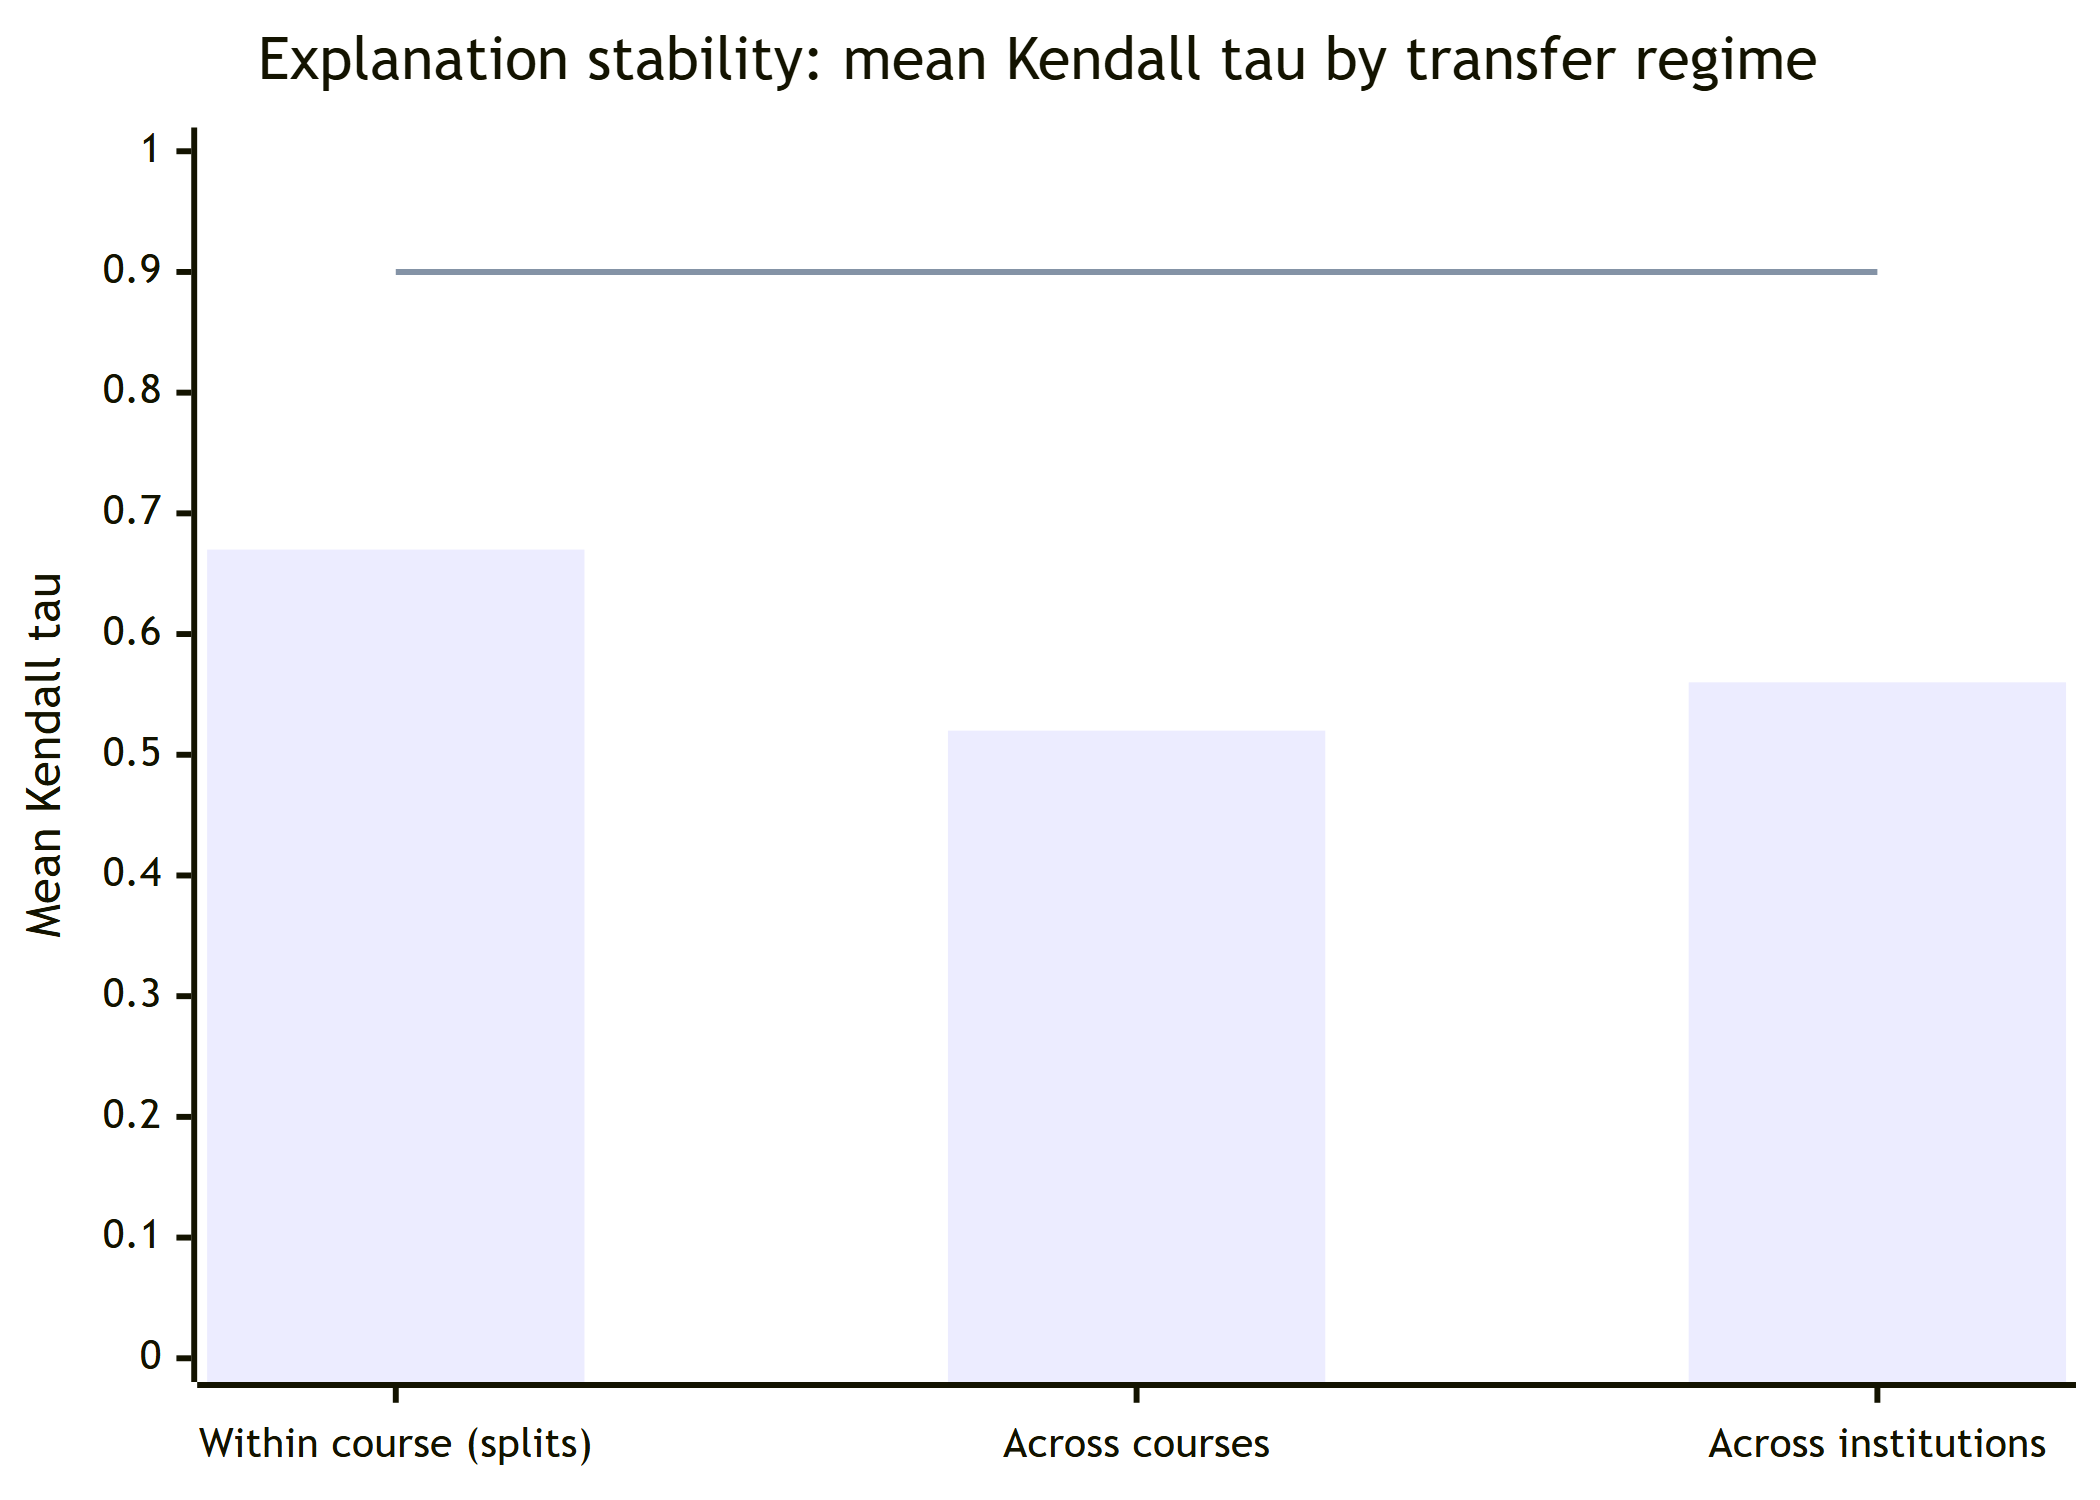
\includegraphics[width=\columnwidth]{figures/fig7_stability.png}
\caption{Explanation-stability summary. Mean Kendall $\tau$ of
permutation-importance rankings falls as the evaluation regime moves further from
training (within-course $\rightarrow$ across-course $\rightarrow$
across-institution) and never reaches the $\tau = 0.90$ stability threshold
(line). Explanations must therefore be framed as model behaviour under a
particular evaluation scenario, not as stable causal rankings.}
\label{fig:stability}
\end{figure}

A controlled synthetic faithfulness probe confirms the method is faithful when
ground truth is known: at the final course week, permutation importance recovers
the generator's weight \emph{ordering} exactly (Kendall $\tau = 1.0$). The same
few features dominate across regimes, but their relative priority reorders --- so
explanations must be framed as model-behaviour under a particular evaluation
scenario, not as stable causal rankings.

\subsection{Second institution}
KU Leuven exposes clickstream and course structure but \textbf{no intermediate
scored assessments and no continuous grade} --- only a binary \texttt{PASSED}
outcome. The mastery/Twin ablation therefore cannot be built there at all (itself
a cross-institution heterogeneity result). On its engagement-only task,
prediction is modest (F1 0.75--0.76, ROC-AUC 0.65--0.72) and a richer engagement
set does not beat a minimal two-feature one (fixed-model F1 delta $-0.015 /
+0.000$). A matched three-institution synthesis confirms a two-feature engagement
baseline (clicks + active-days) is hard to beat (F1 delta spread $-0.016$ to
$+0.026$).

\section{Discussion}
Three points follow. First, on the \textbf{central question} --- do Twin features
beat a competent LMS baseline? --- the honest answer across three real cohorts
and two institutions is \emph{not robustly}. The benefit is real but narrow (BBB,
temporal-forward, mastery) and vanishes under the stricter student-grouped
regime, on other courses, and on other blocks. Reporting only the favourable
cell, as is common, would have manufactured a false ``Twin wins'' narrative.

Second, \textbf{explanations are regime-dependent}. Importance rankings reorder
across splits, courses, and institutions, which has a direct product consequence:
a teacher UI must present XAI output as ``how the model weights each signal for
this prediction'', not ``why this student is at risk''. Our interface encodes
exactly this caveat.

Third, the contribution is best read on \textbf{three axes}, not accuracy alone.
On accuracy this work is comparable to standard baselines and below the published
best (ROC-AUC 0.953 vs.\ 0.993 \cite{lopez2025}) --- expected and not a weakness.
On explainability it provides per-student, background-free perturbation
explanations with documented stability limits. On teacher-facing completeness ---
weekly trajectory, per-student XAI panel, cohort filtering, explicit limitation
notice on real OULAD data --- it is, to our knowledge, the most complete
openly-documented artifact of its kind; we offer it as a design demonstrator
whose presentation of XAI output follows from our stability finding
(Section~\ref{sec:xai}), not as an intervention with demonstrated efficacy.

\section{Limitations and Threats to Validity}
\label{sec:limitations}
\textbf{Synthetic circularity (documented failure mode).} During development, a
synthetic target manufactured an apparent ``mastery win''. The synthetic
\texttt{final\_grade} is a deterministic, noise-free closed-form weighted mean of
the same behaviours the features re-aggregate (week-10 reconstruction error
0.008, correlation 1.000000); the resulting $R^2 \approx 0.99$ and saturated
\texttt{passed} F1 $= 1.000$ are \textbf{algebraic artifacts, not learnable
signal}. We report this explicitly as a cautionary methodological result: a
circular target can fabricate a feature-group advantage that disappears on
genuine data.

\textbf{Partial target circularity on OULAD.} \texttt{final\_weighted\_score} is
partly fed by assessment scores, so the regression results lean somewhat on
within-system accounting; the classification target and VLE clickstream are the
cleaner, exogenous evidence.

\textbf{Mastery redundancy.} \texttt{overall\_mastery} is close to cumulative LMS
performance ($|r| = 0.993$ with \texttt{avg\_assignment\_score}), so it must not
be presented as an independent construct.

\textbf{No user evaluation of the interface.} The teacher interface is a design
demonstrator: its presentation of XAI output as model-behaviour-under-a-scenario
follows directly from the explanation-stability result (Section~\ref{sec:xai}),
but we make no claim about its effect on teacher understanding or decisions. A
qualitative or controlled study with instructors is left to future work.

\textbf{External validity.} Evidence spans two OULAD courses (one institution)
and a second institution that cannot test the mastery ablation; this supports the
narrower claim that feature-richness does not robustly help, not a like-for-like
institutional replication. Explanations are not causal and not SHAP. Intervention
and counterfactual reasoning are out of scope --- the ``Digital Twin'' here is a
state representation, not a simulation engine.

\section{Conclusion}
We presented an explainable, teacher-facing Student Digital Twin and evaluated it
honestly across two institutions. On real, non-circular OULAD data the engineered
Twin features do not deliver a consistent advantage over a competent LMS
baseline: the result is mixed-to-null on DDD 2013J and heterogeneous on BBB 2013J
(mastery $-1.026$ RMSE on temporal-forward only), and a second institution cannot
even build the ablation. The accompanying XAI explanations are regime-sensitive
within a course (Kendall $\tau$ 0.55--0.79) and partly course-specific across
courses (0.32--0.61). The contribution is therefore methodological and
system-level --- a reproducible, leakage-aware pipeline with a teacher interface,
an explanation-stability analysis, a documented synthetic-circularity failure
mode, and an honest multi-cohort finding --- rather than an accuracy record.
Future work includes external validation across more institutions and validated
intervention/counterfactual reasoning.

\section*{Data and Code Availability}
All datasets used are public and openly licensed. OULAD is distributed under
CC-BY 4.0 \cite{kuzilek2017}; the KU Leuven activity/performance dataset is
distributed under CC-BY 4.0 via Zenodo \cite{tiukhova2026}. The authors are not
affiliated with, and report no competing interest in, the dataset providers; both
datasets were obtained from their public releases. All experiment code,
configuration, and frozen result artifacts (versioned JSON/CSV per experiment)
are available in the project repository at \texttt{[[repository URL --- TODO]]}
to support independent reproduction.

\begin{thebibliography}{99}
\bibitem{kuzilek2017} J. Kuzilek, M. Hlosta, and Z. Zdrahal, ``Open University
Learning Analytics dataset,'' \emph{Scientific Data}, vol.~4, art.~170171, 2017,
doi: 10.1038/sdata.2017.171.

\bibitem{tiukhova2024} E. Tiukhova, P. Vemuri, N. L\'opez Flores, A. S. Islind,
M. \'Oskarsd\'ottir, S. Poelmans, B. Baesens, and M. Snoeck, ``Explainable
Learning Analytics: Assessing the stability of student success prediction models
by means of explainable AI,'' \emph{Decision Support Systems}, vol.~182,
art.~114229, 2024, doi: 10.1016/j.dss.2024.114229.

\bibitem{tiukhova2026} E. Tiukhova, D. Van Landuyt, B. Baesens, and M. Snoeck,
``Open data, private learners: a de-identified student activity and performance
dataset for learning analytics,'' \emph{Scientific Data}, 2026, Zenodo,
doi: 10.5281/zenodo.17087849.

\bibitem{lopez2025} J. L\'opez de la Rosa et al., ``A Modular and Explainable
Machine Learning Pipeline for Student Dropout Prediction in Higher Education,''
\emph{Algorithms}, vol.~18, no.~10, art.~662, 2025, doi: 10.3390/a18100662.

\bibitem{review2026} ``Predicting student performance: A comprehensive review of
machine learning, deep learning, and explainable AI approaches,'' \emph{Computers
and Education: Artificial Intelligence}, 2026. [Online]. Available:
\url{https://www.sciencedirect.com/science/article/pii/S2666920X26000093}

\bibitem{xai2025} ``An explainable AI-based approach for predicting undergraduate
students' academic performance,'' \emph{Computers and Education: Artificial
Intelligence}, 2025. [Online]. Available:
\url{https://www.sciencedirect.com/science/article/pii/S2590005625000116}

\bibitem{frontiers2025} ``Machine learning models for academic performance
prediction: interpretability and application in educational decision-making,''
\emph{Frontiers in Education}, vol.~10, art.~1632315, 2025,
doi: 10.3389/feduc.2025.1632315.

\bibitem{dt2022} ``Digital Twins and Artificial Intelligence as Pillars of
Personalized Learning Models,'' \emph{Communications of the ACM}, vol.~65, no.~4,
2022. [Online]. Available:
\url{https://cacm.acm.org/magazines/2022/4/259419}

\bibitem{lundberg2017} S. M. Lundberg and S.-I. Lee, ``A unified approach to
interpreting model predictions,'' in \emph{Advances in Neural Information
Processing Systems (NeurIPS)}, 2017, pp.~4765--4774.

\bibitem{breiman2001} L. Breiman, ``Random forests,'' \emph{Machine Learning},
vol.~45, no.~1, pp.~5--32, 2001, doi: 10.1023/A:1010933404324.

\bibitem{friedman2001} J. H. Friedman, ``Greedy function approximation: a
gradient boosting machine,'' \emph{Annals of Statistics}, vol.~29, no.~5,
pp.~1189--1232, 2001.

\bibitem{kumar2020} I. E. Kumar, S. Venkatasubramanian, C. Scheidegger, and
S. Friedler, ``Problems with Shapley-value-based explanations as feature
importance measures,'' in \emph{Proc. 37th Int. Conf. Machine Learning (ICML)},
2020, pp.~5491--5500.

\bibitem{slack2020} D. Slack, S. Hilgard, E. Jia, S. Singh, and H. Lakkaraju,
``Fooling LIME and SHAP: Adversarial attacks on post hoc explanation methods,''
in \emph{Proc. AAAI/ACM Conf. AI, Ethics, and Society (AIES)}, 2020,
pp.~180--186.
\end{thebibliography}

\end{document}
